%!TEX root = ../Technische Dynamik.tex

\section{Approximation kontinuierlicher Schwinger} % (fold)
	\subsection{Statik des längselastischen Stabes} % (fold)
		\subsubsection{Problem} % (fold)
			Einseitig eingespannter Stab mit gegebener Randverschiebung $u(0) = a$ und gegebener Endlast $F$.
			
			\resizebox{\columnwidth}{!}{
				%!TEX root = ../Technische Dynamik.tex

\tikzstyle{hatch}=[postaction={draw,decorate,decoration={border,angle=-45, amplitude=0.15cm,segment length=1.2mm}}]

\begin{tikzpicture}[>=latex]

\draw[hatch] (0,1) -- (0,-1);
\draw (0,-0.3) rectangle (8,0.3);
\draw (3,0.5) -- (3,-1);
\draw[->] (0,-0.8) -- node[below] {$x$} (3,-0.8);
\draw[dashed] (0,0) -- (0,-1.3);
\draw[dashed] (8,0) -- (8,-1.3);
\node at (0.4,-1.5) {$x=0$};
\node at (8.4,-1.5) {$x=l$};

\draw[->] (3,0) -- (4,0) node[right] {$u(x)$};
\draw[->] (8,0) -- (9.5,0) node[right] {$F$};

\draw (0,0.3) to[out=70,in=200] (0.5,0.8) node[right] {$u(0)=a$};
\draw (6,0) to[out=0,in=180] (6.5,1) node[right] {$EA$};

\end{tikzpicture}
			}
			
			\begin{description}
				\item[Problem:] Finde $u(x)$ so, dass
					\begin{equation} \label{eq:stab_bed}
						\begin{split}
								EAu''(x) &= 0 \\
								u(x=0) &= a \\
								EAu'(l) &= F
						\end{split}
					\end{equation}
				
				\item[Lösung] durch Integration:
					\[
						u(x) = \frac{F}{EA} x + a
					\]
			\end{description}
		% subsubsection Problem (end)
		
		\subsubsection{Behandlung mit virtueller Arbeit} % (fold)
			Zerlege System in Inneres und Rand:
			
			\resizebox{\columnwidth}{!}{
				%!TEX root = ../Technische Dynamik.tex

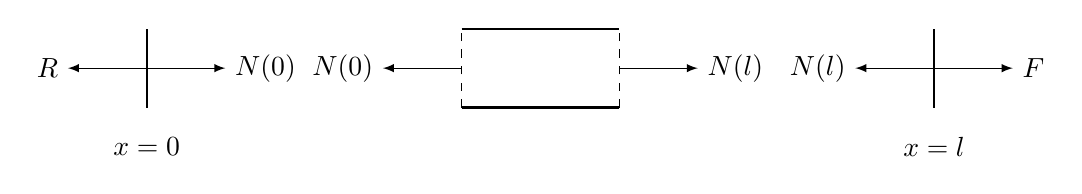
\begin{tikzpicture}[>=latex]
\begin{scope}
	\draw[thick] (0,0) -- (0,1);
	\draw[->] (0,0.5) -- (-1,0.5) node[left] {$R$};
	\draw[->] (0,0.5) -- (1,0.5) node[right] {$N(0)$};

	\node at (0,-0.5) {$x=0$};
\end{scope}

\begin{scope}[xshift=4cm]
	\draw[thick] (0,0) -- (2,0)
	                   (0,1) -- (2,1);
	\draw[dashed] (0,0) -- (0,1)
	                      (2,0) -- (2,1);

	\draw[->] (0,0.5) -- (-1,0.5) node[left] {$N(0)$};
	\draw[->] (2,0.5) -- (3,0.5) node[right] {$N(l)$};
\end{scope}

\begin{scope}[xshift=10cm]
	\draw[thick] (0,0) -- (0,1);
	\draw[->] (0,0.5) -- (-1,0.5) node[left] {$N(l)$};
	\draw[->] (0,0.5) -- (1,0.5) node[right] {$F$};

	\node at (0,-0.5) {$x=l$};
\end{scope}
\end{tikzpicture}
			}
			
			\paragraph{Problem I} % (fold)
				\[
					\mathcal{U} := \{
						u(x) \ | \ u(0) = a
					\} \, , \ 
					\mathcal{V} := \{
						\delta u(x) \ | \ \delta u(0) = 0
					\}
				\]
				
				Finde $u(x) \in \mathcal{U}$ so, dass
				\[
					- \int_0^l \delta u(x) EAu''(x) \diff x - \delta u(l) (F - EAu'(l)) = 0 \quad \forall \: \delta u(x) \in \mathcal{V}
				\]
				Erfüllt \eqref{eq:stab_bed} $\Rightarrow$ \textbf{\ref{subs:residuen} \nameref{subs:residuen}}
			% paragraph Problem I (end)
			
			\paragraph{Problem II} % (fold)
				\[
					\mathcal{U} := \{
						u(x) \ | \ u(0) = a
					\} \, , \ 
					\mathcal{V} := \{
						\delta u(x) \ | \ \delta u(0) = 0
					\}
				\]
			
				Finde $u(x) \in \mathcal{U}$ so, dass
				\[
					\int_0^l \delta u'(x) EAu'(x) \diff x - \delta u(l) F = 0 \quad \forall \: \delta u(x) \in \mathcal{V}
				\]
				Erfüllt \eqref{eq:stab_bed} $\Rightarrow$ \textbf{\ref{subs:galerkin} \nameref{subs:galerkin}}
			% paragraph Problem II (end)
			
			\paragraph{Problem III} % (fold)
				\[
					\mathcal{U} := \{
						u(x) \ | \ u(0) = a
					\}
				\]
			
				Finde die stationären Punkte $u(x) \in \mathcal{U}$ des Variationsproblems
				\[
					I(u) = \half \int_0^l EAu'^{\:2\!}(x) \diff x - u(l) F \longrightarrow \text{stationär + RB}
				\]
				Erfüllt \eqref{eq:stab_bed} $\Rightarrow$ \textbf{\ref{subs:ritz} \nameref{subs:ritz}}
			% paragraph Problem III (end)
		% subsubsection Behandlung mit virtueller Arbeit (end)
		
		\subsubsection{Das Ritz-Verfahren} % (fold)
			\label{subs:ritz}
			Wähle als Ansatz für Näherung $u_n(x)$ $n$-parametrige Schar
			\[
				\mathcal U \supset \mathcal U^n := \left\{
					u_n(x) = \sum_{i=1}^n q_i v_i(x) + p(x) = \vec q^\transp \vec v(x) + p(x)
				\right\}
			\]
			mit:
			\begin{itemize}
				\item[$v_i(x)$:] gewählte Ansatzfunktion mit $v_i(0) = 0$
				\item[$p(x)$:] gewählte Ansatzfunktion mit $p(0) = a$
				\item[$q_i$:] zu bestimmende (Gewichtungs-)Koeffizienten
			\end{itemize}
			\emphequation{equation*}{
				\underbrace{
					\int_0^l EA \vec v'(x) \vec v'^\transp (x) \diff x
				}_K \vec q =
				\underbrace{
					F \vec v(l) - \int_0^l EA \vec v'(x) p'(x) \diff x
				}_\vec{b}
			}
			
			\begin{bemerkung}
				Wenn Ansatz treffen kann, dann trifft er auch.
			\end{bemerkung}
		% subsubsection Das Ritz-Verfahren (end)
		
		\subsubsection{Das Galerkin-Verfahren} % (fold)
			\label{subs:galerkin}
			Wähle für Näherung $u_n(x)$ gleichen Ansatz wie beim Ritz-Verfahren und \emph{zugehöriges} virtuelles Verschiebungsfeld:
			\[
				\mathcal V \supset \mathcal V^n = \left\{
					\delta u_n(x) = \Part{u_n(x)}{\vec q} \delta \vec q = \delta \vec q^\transp \vec v(x)
				\right\}
			\]
			Gleiches Ergebnis wie beim Ritz-Verfahren.
			
			\begin{bemerkungen}
				\item Falls zugehöriges Variationsproblem existiert und das virtuelle Verschiebungsfeld wie oben gewählt wird, sind Ritz und Galerkin Verfahren identisch (Ritz-Galerkin-Verfahren).
				
				\item Finite-Elemente-Methode ist ein Spezialfall des Galerkin-Verfahrens.
			\end{bemerkungen}
		% subsubsection Das Galerkin-Verfahren (end)
		
		\subsubsection{Methode der gewichteten Residuen} % (fold)
			\label{subs:residuen}
			Wähle Ansatz wie beim Galerkin-Verfahren. Somit:
			\emphequation{gather*}{
				EA\parens{
					\vec v(l) \vec v'^\transp (l) - \int_0^l \vec v(x) \vec v''^\transp (x) \diff x
				} \vec q = \\ \hfill \qquad
				- EA \parens{
					\vec v(l) p'(l) - \int_0^l \vec v (x) p''(x) \diff x
				} + \vec v(l) F
			}
			
			\begin{bemerkungen}
				\item Gleiches Ergebnis wie Galerkin-Verfahren, aber höhere Ableitungen von $u_n(x)$ müssen existieren.
				\item \emph{Klassische} gewichtete Residuen: Ansatz muss \emph{zusätzlich} die \emph{statischen} Randbedingungen
					\[
						u_n' (l) = \frac{F}{EA} \quad \forall \: \vec q
					\]
					erfüllen. Damit ist nur noch folgendes zu fordern:
					\[
						0 = - \int_0^l \delta u_n(x) EAu_n''(x) \diff x \quad \forall \: \delta u_n \in \mathcal V^n
					\]
			\end{bemerkungen}
		% subsubsection Methode der gewichteten Residuen (end)
		
		\subsubsection{Zusammenfassung} % (fold)
			\begin{itemize}
				\item Ansatzfunktionen $v_i(x)$ müssen bei allen Methoden \emph{linear unabhängig} sein.
				\item Matrizen der Form $\int \vec v'(x) \vec v'^\transp (x) \diff x$ heissen \emph{Ortsintegralmatrix}.
			\end{itemize}
		% subsubsection Zusammenfassung (end)
	% subsection Statik des längselastischen Stabes (end)
	
	\subsection{Biegeschwingungen von Balken} % (fold)
		\resizebox{\columnwidth}{!}{
			%!TEX root = ../Technische Dynamik.tex

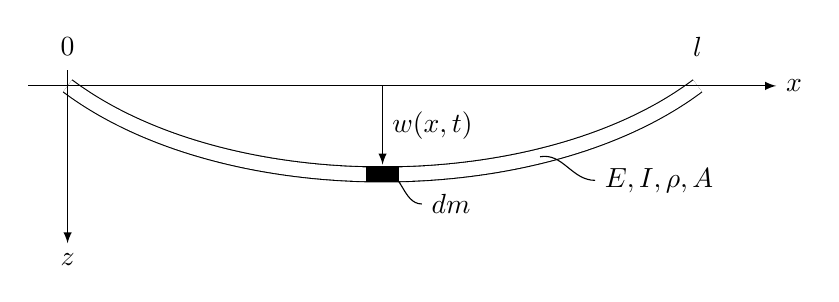
\begin{tikzpicture}[>=latex]
\draw[double distance=5pt] (0,0) .. controls (2,-1.5) and (6,-1.5) .. (8,0);
\draw[fill] (3.8,-1.21) rectangle (4.2,-1.03);
\draw (4,-1.1) to[in=180,out=10] (4.5,-1.5) node[right] {$dm$};
\draw (6,-0.9) to[in=180,out=10] (6.7,-1.2) node[right] {$E,I,\rho,A$};
\draw[->] (4,0) -- node[right] {$w(x,t)$} (4,-1);

\draw[->] (-0.5,0) -- (9,0) node[right]{$x$};
\node at (0,0.5) {$0$};
\node at (8,0.5) {$l$};
\draw[->] (0,0.2) -- (0,-2) node[below]{$z$};
\end{tikzpicture}
		}
		
		\paragraph{Freischneiden} % (fold)
			\begin{align*}
				M(x,t) &= -EI(x)w_{xx}(x,t) \\
				Q(x,t) &= M_x(x,t) \\
				\diff m &= \rho A(x) \diff x
			\end{align*}
			
			Sei $A = \const$ und $I = \const$, so ergibt sich die \emph{partielle Dgl. für Euler-Bernoulli-Balken}:
			\emphequation{equation*}{
				w_{tt}(x,t) = - \frac{EI}{\rho A} w_{xxxx}(x,t)
			}
		
			\begin{center}
				%!TEX root = ../Technische Dynamik.tex

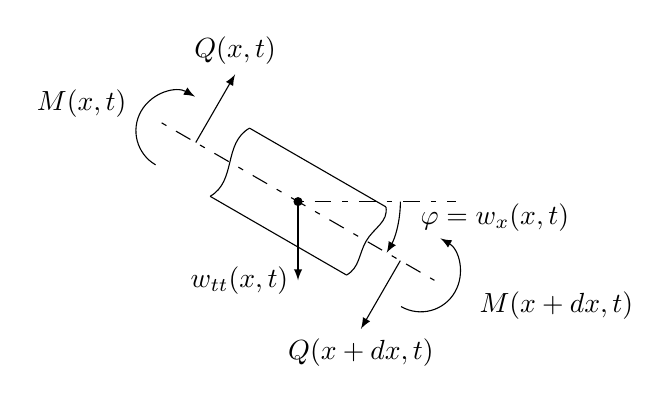
\begin{tikzpicture}[>=latex]
\begin{scope}[rotate=-30]
\draw[dash pattern=on 2pt off 4pt on 6pt off 4pt] (-2,0) -- (2,0);
\draw (-1,-0.5) -- (1,-0.5);
\draw (-1,0.5) -- (1,0.5);
\draw (-1,-0.5) to[in=-120,out=60] (-1,0.5);
\draw (1,-0.5) to[in=-90,out=60] (1,0)  to[in=-50,out=90] (1,0.5);

\draw[->] (-1.5,0) -- (-1.5,1) node[above] {$Q(x,t)$};
\draw[->] (1.5,0) -- (1.5,-1) node[below] {$Q(x+dx,t)$};
\draw[->] (-1.8,-0.5) arc (270:90:0.5);
\node at (-3,-0.3) {$M(x,t)$};
\draw[->] (1.8,-0.5) arc (-90:90:0.5);
\node at (3.5,0.5) {$M(x+dx,t)$};
\end{scope}

\draw[fill] (0,0) circle (0.05);
\draw[->] (0,0) -- (0,-1) node[left] {$w_{tt}(x,t)$};
\draw[dash pattern=on 2pt off 4pt on 6pt off 4pt] (0,0) -- (2,0);

\draw[->] (1.3,0) arc (0:-30:1.3);
\node at (2.5,-0.2) {$\varphi=w_x(x,t)$};
\end{tikzpicture}
			\end{center}
		% paragraph Freischneiden (end)
		
		\paragraph{Lösung mit Separationsansatz} % (fold)
			Sei
			\begin{gather*}
				w(x,t) = v(x)q(t) \quad \Rightarrow \quad w_{tt} = v \ddot q \, , \ w_{xxxx} = v''''q \\
				\beta^4 = \frac{\rho A}{EI} \omega^2
			\end{gather*}
			\emphequation{gather*}{
				v(x) = A\cos(\beta x) + B\sin(\beta x) + C\cosh(\beta x) + D\sinh(\beta x) \\
				\ q(t) = E\sin(\omega t) + F\cos(\omega t)
			}
			Bestimme $A$, $B$, $C$, $D$, $\omega$ aus Einspannung und $E$, $F$ aus Anfangsbedingungen, anschliessend superponieren.
		% paragraph Lösung mit Separationsansatz (end)
		
		\paragraph{Einspannfälle} % (fold)
			\begin{center}
				% \renewcommand{\arraystretch}{}
				\begin{tabular}{cllcc}
					\toprule
					$x = 0$ & Typ & kinem. RB & kinet. RB \\
					\midrule
					\multirow{2}{*}{\resizebox{!}{.75cm}{%!TEX root = ../Technische Dynamik.tex

\tikzstyle{hatch}=[postaction={draw,decorate,decoration={border,angle=-45, amplitude=0.2cm,segment length=1.4mm}}]

\begin{tikzpicture}[>=latex]

\draw[hatch] (-0.5,0) -- (0.5,0);
\draw[fill=white] (0,0.5) circle (0.1);
\draw (-0.3,0) -- (0.3,0) -- (0,.5) -- cycle;

\draw (0,0.4) -- (1.04,0.4);
\draw (0,0.6) -- (.97,0.6);
\draw (1,0.3) to[in=-130,out=40] (1,0.7);

\end{tikzpicture}}} & gelenkige & $w(0,t) = 0$ & \\ 
					 & Lagerung & & $M(0,t) = 0$ \\
					\midrule
					\multirow{2}{*}{\resizebox{!}{.75cm}{%!TEX root = ../Technische Dynamik.tex

\tikzstyle{hatch}=[postaction={draw,decorate,decoration={border,angle=-45, amplitude=0.2cm,segment length=1.4mm}}]

\begin{tikzpicture}[>=latex]
\draw[hatch] (0,0.5) -- (0,0-.5);
\draw (0.1,0.1) -- (.97,0.1);
\draw (0.1,-0.1) -- (1.04,-0.1);
\draw (0.1,-0.3) -- (0.1,0.3);
\draw (1,-0.2) to[in=-130,out=40] (1,0.2);
\end{tikzpicture}}} & lineare & & $Q(0,t) = 0$ \\
					  & Führung & $w_x(0,t) = 0$ & \\
					\midrule
					\multirow{2}{*}{\resizebox{!}{.75cm}{%!TEX root = ../Technische Dynamik.tex

\tikzstyle{hatch}=[postaction={draw,decorate,decoration={border,angle=-45, amplitude=0.2cm,segment length=1.4mm}}]

\begin{tikzpicture}[>=latex]
\draw[hatch] (0,0.5) -- (0,0-.5);
\draw (0,0.1) -- (.97,0.1);
\draw (0,-0.1) -- (1.04,-0.1);
\draw (1,-0.2) to[in=-130,out=40] (1,0.2);
\end{tikzpicture}}} & feste &  $w(0,t) = 0$ & \\
					 & Einspannung & $w_x(0,t) = 0$ & \\
					\midrule
					\multirow{2}{*}{\resizebox{!}{.4cm}{%!TEX root = ../Technische Dynamik.tex

\tikzstyle{hatch}=[postaction={draw,decorate,decoration={border,angle=-45, amplitude=0.2cm,segment length=1.4mm}}]

\begin{tikzpicture}[>=latex]
\draw (0,0.1) -- (0,0-.1);
\draw (0,0.1) -- (.97,0.1);
\draw (0,-0.1) -- (1.04,-0.1);
\draw (1,-0.2) to[in=-130,out=40] (1,0.2);
\end{tikzpicture}}} & freies & & $Q(0,t) = 0$ \\
					 & Ende & & $M(0,t) = 0$ \\
					\bottomrule
				\end{tabular}
			\end{center}
		% paragraph Einspannfälle (end)
	% subsection Biegeschwingungen von Balken (end)
	
	\subsection{Das Ritz-Verfahren für dynamische Probleme} % (fold)
		Ansatz für Näherung $w_n(x,t)$:
		\begin{align*}
			\mathcal W \supset \mathcal W^n = \bigg\{
				\delta w_n(x,t) &= \sum_{i=1}^n q_i(t) v_i(x) + p(x,t) \\
				&= \underbrace{\vec v^\transp(x)}_\text{gegeben} \vec q(t) + \underbrace{p(x,t)}_\text{gegeben}
			\bigg\}
		\end{align*}
		
		\begin{bemerkungen}
			\item Zu bestimmende Koeffizienten $q_i(t)$ sind jetzt \emph{zeitabhängig}.
			\item Ansatz $w_n(x,t)$ muss kinematische Randbedingungen erfüllen $\forall \: \vec q(t)$
		\end{bemerkungen}
		\begin{align*}
			I(w) &= \int \Big( T(w) - V(w) \Big) \diff t \stackrel{!}{\longrightarrow} \text{stationär} \\
			T(w) &= \int_0^l F(x,t,w,w_t,\dots) \diff x \\
			V(w) &= \int_0^l G(x,t,w,w_x,w_{xx}) \diff x
		\end{align*}
		Mit Näherungsansatz ins Funktional:
		\begin{align*}
			I(w_n) &= \int \Big( T(w_n) - V(w_n) \Big) \diff t \\
			&= \int \Big( T_n(t, \vec q, \dot{\vec q}) - V_n(t, \vec q) \Big) \diff t \\
			&= I_n(\vec q) \longrightarrow \text{stationär}
		\end{align*}
		
		Notwendige Bedingung: Lagrange II
		\[
			\Diff{}{t}\parens{\Part{T_n}{\dot{\vec q}}}^{\!\transp\!} - \parens{\Part{T_n}{\vec q}}^{\!\transp\!} + \parens{\Part{V_n}{\vec q}}^{\!\transp\!} = \vec f^\text{NP}
		\]
		führt auf $n$-dimensionales Differentialgleichungssystem
		\[
			\mtrx M(t, \vec q) \ddot{\vec q} - \vec h(t, \vec q, \dot{\vec q}) = 0
		\]
		Löse System $\Rightarrow$ Näherung $w_n(x,t)$ bestimmt.
	% subsection Das Ritz-Verfahren für dynamische Probleme (end)
% section approximation_kontinuierlicher_schwinger (end)
